\documentclass[aspectratio=169]{beamer}
\usetheme{Madrid}
\usecolortheme{default}

\usepackage{amsmath}
\usepackage{amssymb}
\usepackage{graphicx}
\usepackage{booktabs}
\usepackage{xcolor}
\usepackage{listings}
\usepackage{tikz}
\usetikzlibrary{shapes.geometric, arrows.meta, positioning}

\lstset{
    language=Python,
    basicstyle=\ttfamily\scriptsize,
    keywordstyle=\color{blue},
    commentstyle=\color{gray},
    stringstyle=\color{red!70!black},
    breaklines=true,
    showstringspaces=false,
    tabsize=2,
    backgroundcolor=\color{gray!10},
    frame=single,
    framesep=2pt,
    xleftmargin=4pt,
    xrightmargin=4pt
}

\title{Week 8: Deep Learning}
\subtitle{Activation Functions, CNNs, RNNs \& Best Practices}
\author{MDST Project: Heart Failure Survival Analysis}
\date{2026}

\begin{document}

%=============================================================
% TITLE SLIDE
%=============================================================
\frame{\titlepage}

%=============================================================
% TABLE OF CONTENTS
%=============================================================
\begin{frame}{Outline}
\tableofcontents
\end{frame}

%=============================================================
\section{Recap: Perceptron \& MLP}
%=============================================================

\begin{frame}{Recap: From Perceptron to Multi-Layer Perceptron}

\begin{columns}
\column{0.5\textwidth}
\textbf{Perceptron (1958):}
\begin{itemize}
    \item Single neuron: $\hat{y} = \sigma(\mathbf{w}^\top \mathbf{x} + b)$
    \item Can only learn \textbf{linearly separable} patterns
    \item Binary step activation: 0 or 1
\end{itemize}

\vspace{0.3cm}
\textbf{Limitation:} Cannot solve XOR --- proved to kill neural net research in 1969!

\column{0.5\textwidth}
\textbf{Multi-Layer Perceptron (MLP):}
\begin{itemize}
    \item Stack multiple layers of neurons
    \item \textbf{Hidden layers} learn intermediate representations
    \item With non-linear activations: \emph{universal function approximator}
\end{itemize}

\vspace{0.3cm}
\textbf{Key insight:} Depth + non-linearity = power to learn \emph{any} function
\end{columns}

\vspace{0.3cm}
\centering
\textbf{Forward pass:} $\mathbf{h}^{(l)} = \sigma\!\left(\mathbf{W}^{(l)}\mathbf{h}^{(l-1)} + \mathbf{b}^{(l)}\right)$
\end{frame}

%=============================================================
\section{Activation Functions}
%=============================================================

\begin{frame}{Activation Functions: Why They Matter}

Without non-linear activations, stacking layers collapses to a single linear transformation:
\[
\mathbf{W}_3(\mathbf{W}_2(\mathbf{W}_1\mathbf{x})) = \mathbf{W}_{\text{eff}}\mathbf{x} \quad \longrightarrow \text{still linear!}
\]

\vspace{0.3cm}
\textbf{Activation function} $\sigma$ introduces non-linearity between layers.

\vspace{0.3cm}
\begin{columns}
\column{0.55\textwidth}
\textbf{Desirable properties:}
\begin{itemize}
    \item Non-linear
    \item Differentiable (for backprop)
    \item Doesn't saturate (avoids vanishing gradients)
    \item Computationally cheap
\end{itemize}

\column{0.45\textwidth}
\textbf{Common choices:}
\begin{itemize}
    \item \textbf{ReLU} --- hidden layers
    \item \textbf{Sigmoid} --- binary output
    \item \textbf{Softmax} --- multi-class output
    \item \textbf{Tanh} --- zero-centered
\end{itemize}
\end{columns}
\end{frame}

\begin{frame}{Activation Functions: Formulas \& Trade-offs}

\small
\begin{tabular}{@{}lllll@{}}
\toprule
\textbf{Activation} & \textbf{Formula} & \textbf{Range} & \textbf{Pros} & \textbf{Cons} \\
\midrule
\textbf{Sigmoid} & $\sigma(z) = \tfrac{1}{1+e^{-z}}$ & $(0,1)$ & Probability output & Vanishing gradients \\[4pt]
\textbf{Tanh} & $\tanh(z) = \tfrac{e^z - e^{-z}}{e^z + e^{-z}}$ & $(-1,1)$ & Zero-centered & Vanishing gradients \\[4pt]
\textbf{ReLU} & $f(z) = \max(0,z)$ & $[0,\infty)$ & Fast, no saturation & Dead neurons \\[4pt]
\textbf{Leaky ReLU} & $f(z) = \max(\alpha z,\, z)$, $\alpha{\approx}0.01$ & $(-\infty,\infty)$ & No dead neurons & Slight overhead \\[4pt]
\textbf{ELU} & $f(z) = \begin{cases} z & z{>}0 \\ \alpha(e^z{-}1) & z{\le}0 \end{cases}$ & $(-\alpha,\infty)$ & Smooth, mean $\approx 0$ & Slight overhead \\
\bottomrule
\end{tabular}

\vspace{0.4cm}
\begin{block}{Practical Recommendation}
\textbf{Hidden layers:} start with ReLU \quad
\textbf{Output (binary):} sigmoid \quad
\textbf{Output (multi-class):} softmax
\end{block}
\end{frame}

\begin{frame}{Vanishing Gradient Problem}

\begin{columns}
\column{0.55\textwidth}
\textbf{What happens during backprop?}

\[
\frac{\partial \mathcal{L}}{\partial \mathbf{W}^{(1)}} = \frac{\partial \mathcal{L}}{\partial \mathbf{h}^{(L)}} \cdot \prod_{l=2}^{L} \frac{\partial \mathbf{h}^{(l)}}{\partial \mathbf{h}^{(l-1)}}
\]

Each term includes $\sigma'(z)$. For sigmoid/tanh:
\begin{itemize}
    \item $\sigma'(z) \le 0.25$ (sigmoid), $\le 1$ (tanh)
    \item Product of many small values $\to 0$
    \item \textbf{Early layers get no gradient}
\end{itemize}

\column{0.45\textwidth}
\textbf{Why ReLU helps:}
\[
\text{ReLU}'(z) = \begin{cases} 1 & z > 0 \\ 0 & z \le 0 \end{cases}
\]

\begin{itemize}
    \item Gradient = 1 when active
    \item No squashing for positive values
    \item \textbf{Dead neuron}: if $z \le 0$ always, gradient = 0 forever
    \item Fix: Leaky ReLU ($\alpha z$ instead of 0)
\end{itemize}
\end{columns}
\end{frame}

%=============================================================
\section{Regularization}
%=============================================================

\begin{frame}{The Overfitting Problem}

\begin{columns}
\column{0.5\textwidth}
\textbf{Bias-Variance Trade-off:}

\vspace{0.2cm}
\begin{tabular}{@{}lll@{}}
\toprule
\textbf{State} & \textbf{Train} & \textbf{Test} \\
\midrule
Underfitting & Poor & Poor \\
Good fit & Good & Good \\
Overfitting & Excellent & Poor \\
\bottomrule
\end{tabular}

\vspace{0.4cm}
\textbf{Regularization} adds a penalty term to the loss to discourage overly complex models.

\column{0.5\textwidth}
\textbf{Main regularization strategies:}
\begin{enumerate}
    \item \textbf{L1 / L2} weight penalties
    \item \textbf{Dropout} --- random neuron masking
    \item \textbf{Early Stopping} --- monitor val loss
    \item \textbf{Batch Normalization} --- stabilize activations
    \item \textbf{Data augmentation} (more data)
\end{enumerate}
\end{columns}
\end{frame}

\begin{frame}{L1 and L2 Regularization}

\begin{columns}
\column{0.5\textwidth}
\textbf{L2 Regularization (Weight Decay):}
\[
\mathcal{L}_{\text{total}} = \mathcal{L}_{\text{task}} + \lambda \sum_i w_i^2
\]
\begin{itemize}
    \item Penalizes \emph{large} weights uniformly
    \item Shrinks all weights toward zero
    \item Weights rarely become exactly zero
    \item Default choice; often called \texttt{weight\_decay}
\end{itemize}

\column{0.5\textwidth}
\textbf{L1 Regularization (Lasso):}
\[
\mathcal{L}_{\text{total}} = \mathcal{L}_{\text{task}} + \lambda \sum_i |w_i|
\]
\begin{itemize}
    \item Creates \textbf{sparsity}: drives weights to exactly zero
    \item Acts as implicit \textbf{feature selection}
    \item Useful when many features are irrelevant
\end{itemize}

\vspace{0.2cm}
\textbf{Elastic Net:} $\lambda_1 \|\mathbf{w}\|_1 + \lambda_2 \|\mathbf{w}\|_2^2$ --- combines both
\end{columns}

\vspace{0.3cm}
\begin{block}{Rule of thumb}
$\lambda$ too small $\to$ no effect. \;$\lambda$ too large $\to$ underfitting. Tune with cross-validation.
\end{block}
\end{frame}

\begin{frame}{Dropout}

\textbf{Idea:} During each training step, randomly \emph{zero out} neurons with probability $p$.

\begin{columns}
\column{0.5\textwidth}
\textbf{How it works:}
\begin{itemize}
    \item Each neuron independently masked: $m_i \sim \text{Bernoulli}(1-p)$
    \item Forward pass: $\tilde{\mathbf{h}} = \mathbf{m} \odot \mathbf{h}$
    \item Gradients only flow through unmasked neurons
    \item At \textbf{test time}: use all neurons, scale by $(1-p)$
\end{itemize}

\vspace{0.2cm}
\textbf{Typical rates:}
\begin{itemize}
    \item Fully connected: $p = 0.5$
    \item CNNs: $p = 0.3$
    \item Reduce if underfitting
\end{itemize}

\column{0.5\textwidth}
\textbf{Why it works:}
\begin{enumerate}
    \item Forces \textbf{redundant representations}: no single neuron can dominate
    \item Equivalent to training $2^n$ thinned networks and averaging
    \item Acts as an \textbf{ensemble method}
    \item Prevents co-adaptation of neurons
\end{enumerate}

\vspace{0.3cm}
\begin{block}{In PyTorch}
\texttt{nn.Dropout(p=0.5)} \\
Place \emph{after} activation, \emph{before} next layer
\end{block}
\end{columns}
\end{frame}

\begin{frame}{Batch Normalization \& Early Stopping}

\begin{columns}
\column{0.5\textwidth}
\textbf{Batch Normalization:}
\[
\hat{x}_i = \frac{x_i - \mu_B}{\sqrt{\sigma_B^2 + \epsilon}} \cdot \gamma + \beta
\]

\vspace{0.2cm}
\begin{itemize}
    \item Normalizes each layer's inputs to $\approx \mathcal{N}(0,1)$
    \item $\gamma, \beta$ are \emph{learned} (preserves representational power)
    \item Allows \textbf{higher learning rates}
    \item Reduces sensitivity to initialization
    \item Acts as a regularizer (adds training noise)
\end{itemize}

\column{0.5\textwidth}
\textbf{Early Stopping:}

\vspace{0.2cm}
\begin{itemize}
    \item Monitor \textbf{validation loss} each epoch
    \item If val loss increases for $N$ consecutive epochs: \textbf{stop}
    \item Restore weights from best checkpoint
    \item Simple yet very effective
\end{itemize}

\vspace{0.3cm}
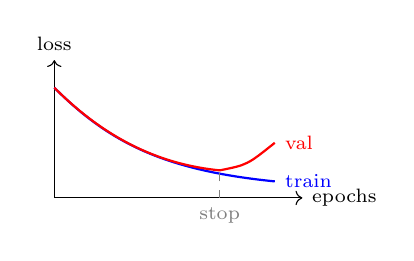
\begin{tikzpicture}[scale=0.7]
    \draw[->] (0,0) -- (4.5,0) node[right] {\scriptsize epochs};
    \draw[->] (0,0) -- (0,2.5) node[above] {\scriptsize loss};
    \draw[blue,thick] (0,2) .. controls (1,1) and (2,0.5) .. (4,0.3) node[right] {\scriptsize train};
    \draw[red,thick] (0,2) .. controls (1,1) and (2,0.6) .. (3,0.5) .. controls (3.5,0.6) .. (4,1.0) node[right] {\scriptsize val};
    \draw[dashed,gray] (3,0) node[below] {\scriptsize stop} -- (3,0.5);
\end{tikzpicture}
\end{columns}
\end{frame}

%=============================================================
\section{Convolutional Neural Networks}
%=============================================================

\begin{frame}{What is a CNN?}

\textbf{CNNs} exploit \textbf{spatial/local structure} in data using two key ideas:

\begin{columns}
\column{0.5\textwidth}
\textbf{1. Local Connectivity (Receptive Fields)}
\begin{itemize}
    \item Each neuron connects to a \emph{small local region}
    \item Not all inputs --- reduces parameters massively
    \item Nearby inputs share more context
\end{itemize}

\vspace{0.3cm}
\textbf{2. Weight Sharing}
\begin{itemize}
    \item Same filter (kernel) applied \emph{everywhere}
    \item A filter detecting an edge works anywhere in the image
    \item $3{\times}3$ filter $\times$ 64 filters = \textbf{576} params (vs millions for FC)
\end{itemize}

\column{0.5\textwidth}
\textbf{3. Hierarchical Feature Learning}
\begin{itemize}
    \item Layer 1: edges, textures
    \item Layer 2: corners, curves
    \item Layer 3+: faces, objects, patterns
\end{itemize}

\vspace{0.3cm}
\textbf{CNN for Heart Failure?}

Tabular data reshaped as \textbf{1D sequence}:
\begin{itemize}
    \item Each feature $\to$ one channel
    \item Local feature interactions (e.g., ejection fraction + creatinine)
    \item Use \texttt{Conv1d} layers
\end{itemize}
\end{columns}
\end{frame}

\begin{frame}{CNN Architecture Components}

\begin{columns}
\column{0.33\textwidth}
\textbf{Convolutional Layer:}
\begin{itemize}
    \item Apply $K$ filters of size $k$
    \item Each filter detects one pattern type
    \item Output: $K$ feature maps
    \item Learned parameters: $K \times k \times C_{\text{in}}$
\end{itemize}

\column{0.33\textwidth}
\textbf{Pooling Layer:}
\begin{itemize}
    \item \textbf{Max pool}: largest activation wins
    \item \textbf{Avg pool}: smooth features
    \item Reduces spatial size
    \item Translation invariance
    \item No learnable parameters
\end{itemize}

\column{0.33\textwidth}
\textbf{Fully Connected Layer:}
\begin{itemize}
    \item Standard linear layer
    \item At the \emph{end} of the CNN
    \item Combines all learned features
    \item Outputs class logits
\end{itemize}
\end{columns}

\vspace{0.4cm}
\textbf{Typical 1D CNN for tabular data:}
\[
\text{Input} \to \underbrace{\text{Conv1d} \to \text{BN} \to \text{ReLU}}_{\times n} \to \text{AdaptiveMaxPool} \to \text{Flatten} \to \text{Linear}
\]
\end{frame}

\begin{frame}{How Convolutions Work: Receptive Field}

\textbf{Receptive field}: the input region that influences one output neuron.

\vspace{0.3cm}
\begin{columns}
\column{0.55\textwidth}
\textbf{1D Example} (kernel size = 3):
\begin{center}
\ttfamily\small
\begin{tabular}{ccccc}
Input: & [1] & [2] & [3] & [4] \\
Filter: & [a] & [b] & [c] & \\
Output $y_1$: & \multicolumn{3}{c}{$a{\cdot}1 + b{\cdot}2 + c{\cdot}3$} \\
\end{tabular}
\end{center}

\vspace{0.3cm}
\textbf{Stacking layers} grows the receptive field:
\begin{itemize}
    \item Layer 1 ($k=3$): RF = 3
    \item Layer 2 ($k=3$): RF = 5
    \item Layer 3 ($k=3$): RF = 7
\end{itemize}

\column{0.45\textwidth}
\textbf{Parameter efficiency:}

Detecting a $7{\times}7$ pattern:
\begin{itemize}
    \item Fully connected: \textbf{49} parameters per output
    \item 3 CNN layers ($k{=}3$): $3\times9 = \textbf{27}$ parameters
\end{itemize}

\vspace{0.3cm}
\textbf{Key formula:}
\[
\text{RF}_l = \text{RF}_{l-1} + (k-1)
\]
\end{columns}
\end{frame}

\begin{frame}{CNN Historical Milestones}

\begin{tabular}{@{}lllp{5cm}@{}}
\toprule
\textbf{Year} & \textbf{Model} & \textbf{Authors} & \textbf{Key Innovation} \\
\midrule
1998 & LeNet-5 & LeCun et al. & Conv + pooling + FC; first practical CNN \\
2012 & AlexNet & Krizhevsky et al. & Deep CNN + ReLU + dropout; won ImageNet \\
2014 & VGGNet & Simonyan \& Zisserman & Depth matters: 16--19 layers of $3{\times}3$ \\
2014 & GoogLeNet & Szegedy et al. & Inception modules; multi-scale features \\
2015 & ResNet & He et al. & \textbf{Skip connections}; enabled 152 layers \\
2016 & DenseNet & Huang et al. & Dense connections; feature reuse \\
2019 & EfficientNet & Tan \& Le & Compound scaling for mobile/edge \\
\bottomrule
\end{tabular}

\vspace{0.4cm}
\begin{block}{Key Takeaway}
Modern CNNs use \textbf{skip connections} because gradient flow matters more than raw depth. ResNet's identity shortcut: $\mathbf{h}^{(l+1)} = \mathcal{F}(\mathbf{h}^{(l)}) + \mathbf{h}^{(l)}$
\end{block}
\end{frame}

%=============================================================
\section{Recurrent Neural Networks}
%=============================================================

\begin{frame}{Why RNNs? The Sequence Modeling Problem}

\textbf{MLPs have fixed-size inputs} and no notion of time. But many problems are sequential:

\begin{columns}
\column{0.5\textwidth}
\textbf{Examples of sequential data:}
\begin{itemize}
    \item Text: ``The cat sat...'' (order critical)
    \item Time series: stock prices, ECG signals
    \item Speech: audio frames
    \item DNA: nucleotide sequences
    \item Patient history: medical records over time
\end{itemize}

\column{0.5\textwidth}
\textbf{What RNNs add:}
\begin{itemize}
    \item \textbf{Hidden state} $h_t$ carries memory across timesteps
    \item \textbf{Parameter sharing} across time: same $W$ at every step
    \item Handles \textbf{variable-length} sequences
\end{itemize}

\vspace{0.3cm}
\textbf{For heart failure:}
Patient records over time form a temporal sequence; earlier measurements predict future outcomes.
\end{columns}
\end{frame}

\begin{frame}{Vanilla RNN: Core Equations}

\begin{columns}
\column{0.5\textwidth}
\textbf{Forward pass at each timestep $t$:}
\[
h_t = \tanh\!\bigl(W_{ih}\, x_t + W_{hh}\, h_{t-1} + b_h\bigr)
\]
\[
y_t = W_{hy}\, h_t + b_y
\]

Where:
\begin{itemize}
    \item $x_t$ = input at time $t$
    \item $h_t$ = hidden state (memory)
    \item $W_{ih}, W_{hh}, W_{hy}$ = \textbf{shared} weights
\end{itemize}

\column{0.5\textwidth}
\textbf{Vanishing Gradient Problem:}

BPTT unrolls the RNN through time:
\[
\frac{\partial h_t}{\partial h_{t-1}} = W_{hh}^\top \cdot \tanh'(\cdots)
\]

For $T$ timesteps, the gradient involves:
\[
\prod_{i=1}^{T} \frac{\partial h_i}{\partial h_{i-1}} = W_{hh}^T \cdot \prod \tanh'
\]

\begin{itemize}
    \item $|W_{hh}| < 1$: gradients \textbf{vanish}
    \item $|W_{hh}| > 1$: gradients \textbf{explode}
    \item Long-range dependencies are lost
\end{itemize}
\end{columns}
\end{frame}

\begin{frame}{LSTM: Long Short-Term Memory}

\textbf{Key idea}: Use multiplicative \emph{gates} to control information flow, with a separate cell state $C_t$ that avoids gradient squashing.

\vspace{0.2cm}
\begin{columns}
\column{0.55\textwidth}
\textbf{LSTM Gate Equations:}

\vspace{0.1cm}
{\small
\begin{align*}
f_t &= \sigma(W_f \cdot [h_{t-1}, x_t] + b_f) \quad &\text{Forget gate}\\
i_t &= \sigma(W_i \cdot [h_{t-1}, x_t] + b_i) \quad &\text{Input gate}\\
\tilde{C}_t &= \tanh(W_c \cdot [h_{t-1}, x_t] + b_c) \quad &\text{Candidate}\\
C_t &= f_t \odot C_{t-1} + i_t \odot \tilde{C}_t \quad &\text{Cell state}\\
o_t &= \sigma(W_o \cdot [h_{t-1}, x_t] + b_o) \quad &\text{Output gate}\\
h_t &= o_t \odot \tanh(C_t) \quad &\text{Hidden state}
\end{align*}
}

\column{0.45\textwidth}
\textbf{Why it works:}
\begin{itemize}
    \item $C_t$ updated with \textbf{addition} (not product) $\to$ gradient highway
    \item $f_t \approx 1$: cell state preserved $\to$ no vanishing
    \item $f_t \approx 0$: old info forgotten (selective)
    \item Gates are \emph{soft} (0--1), learned from data
\end{itemize}

\vspace{0.2cm}
\textbf{Gradient flow via $C_t$:}
\[
\frac{\partial C_t}{\partial C_{t-1}} = f_t \approx 1
\]
\end{columns}
\end{frame}

\begin{frame}{GRU: Gated Recurrent Unit}

\textbf{Simpler alternative to LSTM}: combines forget + input into a single \emph{update gate}.

\begin{columns}
\column{0.55\textwidth}
\textbf{GRU Equations:}

\vspace{0.2cm}
{\small
\begin{align*}
r_t &= \sigma(W_r \cdot [h_{t-1}, x_t] + b_r) \quad &\text{Reset gate}\\
z_t &= \sigma(W_z \cdot [h_{t-1}, x_t] + b_z) \quad &\text{Update gate}\\
\tilde{h}_t &= \tanh(W \cdot [r_t \odot h_{t-1},\, x_t] + b) \quad &\text{Candidate}\\
h_t &= (1 - z_t) \odot h_{t-1} + z_t \odot \tilde{h}_t \quad &\text{Output}
\end{align*}
}

\column{0.45\textwidth}
\textbf{GRU vs LSTM:}

\begin{tabular}{@{}lll@{}}
\toprule
 & \textbf{LSTM} & \textbf{GRU} \\
\midrule
Gates & 3 & 2 \\
States & $h_t, C_t$ & $h_t$ \\
Params & More & Fewer \\
Performance & Similar & Similar \\
Best when & Large data & Small data \\
\bottomrule
\end{tabular}

\vspace{0.3cm}
\textbf{Rule of thumb:} Start with LSTM; use GRU if data is limited or speed matters.
\end{columns}
\end{frame}

\begin{frame}{RNN Architectures for Different Tasks}

\begin{tabular}{@{}lll p{5.5cm}@{}}
\toprule
\textbf{Task type} & \textbf{Architecture} & \textbf{Input$\to$Output} & \textbf{Example} \\
\midrule
Classification & Many-to-one & Sequence $\to$ label & Sentiment analysis, health risk \\
Seq labeling & Many-to-many & Sequence $\to$ sequence & Named entity recognition \\
Translation & Encoder-decoder & Sequence $\to$ sequence & Machine translation \\
Language model & Many-to-many & Token $\to$ next token & Text generation, GPT \\
\bottomrule
\end{tabular}

\vspace{0.4cm}
\begin{columns}
\column{0.5\textwidth}
\textbf{Attention Mechanism (2014):}

Allow decoder to attend to all encoder states:
\[
\text{Attention}(Q, K, V) = \text{softmax}\!\left(\frac{QK^\top}{\sqrt{d_k}}\right) V
\]
\begin{itemize}
    \item Q = Query (what do I need?)
    \item K = Key (what can I offer?)
    \item V = Value (actual information)
\end{itemize}

\column{0.5\textwidth}
\textbf{Transformer (2017):}
\begin{itemize}
    \item Self-attention \emph{without recurrence}
    \item Fully parallel computation
    \item Solves long-range dependency
    \item Foundation of BERT, GPT, T5
\end{itemize}

\vspace{0.2cm}
\textbf{Trend:} Transformers are replacing RNNs even for sequence tasks.
\end{columns}
\end{frame}

%=============================================================
\section{MLP vs CNN vs LSTM: Comparison}
%=============================================================

\begin{frame}{Model Comparison: MLP vs CNN vs LSTM}

\begin{tabular}{@{}lp{2.8cm}p{3cm}p{3.5cm}@{}}
\toprule
 & \textbf{MLP} & \textbf{CNN} & \textbf{LSTM} \\
\midrule
\textbf{Input type} & Fixed-size vectors & Spatial / sequential & Temporal sequences \\
\textbf{Key inductive bias} & None & Local patterns, translation invariance & Temporal ordering, long-range memory \\
\textbf{Parameter sharing} & None & Across spatial positions & Across timesteps \\
\textbf{Depth vs cost} & Quadratic growth & Efficient via convolutions & Sequential; hard to parallelize \\
\textbf{Heart failure use} & Tabular features & Local feature interactions & Patient history over time \\
\textbf{Complexity} & Low--Medium & Medium--High & High \\
\bottomrule
\end{tabular}

\vspace{0.4cm}
\begin{block}{For this dataset}
\textbf{Baseline:} Logistic Regression $\to$ Random Forest $\to$ \textbf{MLP}\\
\textbf{Only escalate} to CNN/LSTM if MLP underperforms and you have reason to believe local or temporal structure exists.
\end{block}
\end{frame}

%=============================================================
\section{Best Practices}
%=============================================================

\begin{frame}{Hyperparameter Selection Strategy}

\begin{columns}
\column{0.5\textwidth}
\textbf{Learning Rate} (most critical):
\begin{itemize}
    \item Too small: very slow convergence
    \item Too large: loss oscillates / diverges
    \item \textbf{Start}: \texttt{lr=0.001}
    \item Use learning rate schedulers
\end{itemize}

\vspace{0.3cm}
\textbf{Batch Size:}
\begin{itemize}
    \item Small (16--32): noisy gradients, regularizes
    \item Large (256+): stable gradients, sharp minima
    \item \textbf{Sweet spot}: 32--128
\end{itemize}

\column{0.5\textwidth}
\textbf{Architecture:}
\begin{itemize}
    \item Start with 1--2 hidden layers
    \item Try $2\times$--$4\times$ \# features in hidden layer
    \item Double \emph{width} before doubling \emph{depth}
\end{itemize}

\vspace{0.3cm}
\textbf{Dropout:}
\begin{itemize}
    \item FC layers: $p = 0.5$
    \item CNNs: $p = 0.3$
    \item Reduce if underfitting
    \item Increase if overfitting
\end{itemize}
\end{columns}
\end{frame}

\begin{frame}{Training Checklist \& Debugging}

\begin{columns}
\column{0.5\textwidth}
\textbf{Before / During Training:}
\begin{itemize}
    \item[$\square$] Normalize inputs (StandardScaler)
    \item[$\square$] Stratified train/val/test splits
    \item[$\square$] Plot loss \& accuracy curves
    \item[$\square$] Tune on \emph{validation set only}
    \item[$\square$] Save checkpoint on best val loss
    \item[$\square$] Evaluate test set \textbf{once at the end}
\end{itemize}

\column{0.5\textwidth}
\textbf{Common Issues:}

{\scriptsize
\begin{tabular}{@{}p{2cm}p{2.2cm}p{2.5cm}@{}}
\toprule
\textbf{Problem} & \textbf{Likely Cause} & \textbf{Fix} \\
\midrule
Loss is NaN & LR too high & Decrease LR, clip gradients \\
Loss not decreasing & LR too low & Increase LR, check normalization \\
Train$\downarrow$ Val$\uparrow$ & Overfitting & Dropout, L2, early stop \\
Loss oscillates & Batch too small & Bigger batch, lower LR \\
Val plateaus & Underfitting & More layers, longer training \\
\bottomrule
\end{tabular}
}
\end{columns}

\vspace{0.3cm}
\begin{block}{Karpathy's Recipe}
Start simple. Overfit one batch first (sanity check). Then regularize. Then scale.
\end{block}
\end{frame}

\begin{frame}{Start Simple, Add Complexity Gradually}

\textbf{Recommended workflow (Karpathy \& Google ML best practices):}

\vspace{0.3cm}
\begin{enumerate}
    \item \textbf{Understand the data}: distributions, outliers, missing values, class balance
    \item \textbf{Baseline}: Logistic Regression --- can humans solve this? Is there signal?
    \item \textbf{Simple non-linear}: Random Forest or Gradient Boosting
    \item \textbf{MLP (2--3 layers)}: moderate non-linearity, fewer assumptions
    \item \textbf{CNN} (if local feature interactions are plausible)
    \item \textbf{LSTM} (only if temporal structure exists)
\end{enumerate}

\vspace{0.3cm}
\begin{columns}
\column{0.6\textwidth}
\begin{block}{Complexity ladder for heart failure dataset}
\texttt{Logistic Regression} $\to$ \texttt{RF/LightGBM} $\to$ \texttt{MLP} $\to$ \texttt{CNN1D} $\to$ \texttt{LSTM}
\end{block}

\column{0.4\textwidth}
\textbf{When to stop climbing:}
\begin{itemize}
    \item When val metric stops improving
    \item When added complexity doesn't justify gains
    \item When you can't explain \emph{why} the fancier model should help
\end{itemize}
\end{columns}
\end{frame}

%=============================================================
% SUMMARY
%=============================================================

\begin{frame}{Summary: Week 8}

\begin{columns}
\column{0.5\textwidth}
\textbf{Key Concepts Covered:}

\vspace{0.2cm}
\begin{itemize}
    \item[\checkmark] \textbf{Activation functions}: ReLU, sigmoid, tanh --- why non-linearity matters
    \item[\checkmark] \textbf{Vanishing gradients}: why sigmoid fails deep, why ReLU helps
    \item[\checkmark] \textbf{Regularization}: L1/L2, dropout, batch norm, early stopping
    \item[\checkmark] \textbf{CNNs}: local connectivity, weight sharing, pooling
    \item[\checkmark] \textbf{RNNs/LSTMs}: hidden state, vanishing gradient solution via gating
    \item[\checkmark] \textbf{Best practices}: start simple, train checklist, debugging
\end{itemize}

\column{0.5\textwidth}
\textbf{Formulas to Remember:}

\vspace{0.2cm}
\begin{tabular}{@{}ll@{}}
\toprule
\textbf{Concept} & \textbf{Formula} \\
\midrule
ReLU & $\max(0, z)$ \\
L2 loss & $\mathcal{L} + \lambda\|\mathbf{w}\|_2^2$ \\
Dropout & $\tilde{h} = m \odot h,\ m \sim \text{Bern}$ \\
LSTM cell & $C_t = f_t \odot C_{t-1} + i_t \odot \tilde{C}_t$ \\
Attention & $\text{softmax}(QK^\top/\sqrt{d_k})\,V$ \\
\bottomrule
\end{tabular}

\vspace{0.4cm}
\textbf{This week's task:} Implement MLP, CNN, LSTM on heart failure dataset and compare.
\end{columns}
\end{frame}

\end{document}
